% пятая часть

\section{Тестирование программы}
Проверяем основной функционал программы. Добавляем новый контроллер, в postgreSQL и FireBird появилось новое оборудование, перед этим прошла проверка на уникальность серийного номера. При редактировании параметров контроллера, данные в базе данных тоже синхронизируются. При проверки таблицы приборов учета проблем не обнаружено.
Список контроллеров и приборов учета полностью совпадает с данными в основной базе данных. 

Производим замену КПУ, это сложный процесс включающий в себе полный перенос всех приборов учета с одного контроллера на другой, в двух базах данных. Для этого нажимаем «Замена».(рисунок~\ref{fig:zamena})
\begin{figure}[H]
	\centering
	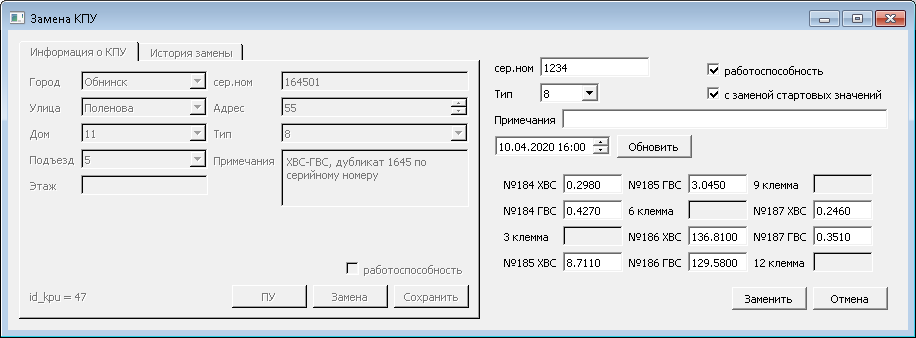
\includegraphics[width=0.9\linewidth]{pics/zamena}
	\caption{Пример замены КПУ}
	\label{fig:zamena}
\end{figure}
При этом вкладка история замены не активна, серийный номер и тип КПУ обязательны для заполнения. Время замены устанавливается автоматически. Если при подготовке нового КПУ установили импульсы такие же, какие и были на старом КПУ, то убираем галочку «с заменой стартовых значений». Выбираем дату и время замены КПУ. Автоматически отображаются номера квартир и показания импульсов приборов учета подключенных к контроллеру. Процесс замены прошел успешно.

В ходе тестирования была выявлена проблема, при постоянном обновлении таблицы начинает подвисать программа. Происходило это из-за обновления данных в выпадающих списках в строке с фильтрами. Метод, который заполняет чек боксы, вызывался не правильно. Данную проблему устранил. Скорость загрузки данных в таблице программы совпадает со скоростью загрузки данных из PostgreSQL.

Сортировка столбца в таблице по значению номера дома происходила не корректно. В номере дома может присутствовать буква, из-за этого в базе данных значение номера дома хранится в формате char. Сортировку производил при запросе данных из базы данных. Поэтому добавил замену формата переменной на integer, если в тексте содержится цифра.
\begin{MyCode}
ORDER BY city.city_name DESC, street.street_name DESC,
cast(substring(house.house_number from \'^[0-9]+\') as integer),
cast(entrance.num_entr as integer) DESC, 
flat.num_flat DESC, counter.type_counter DESC
\end{MyCode}
Во вкладке анализ данных отображаются автоматически выявленные проблемные счетчики. (рисунок~\ref{fig:3})
\begin{figure}[H]
	\centering
	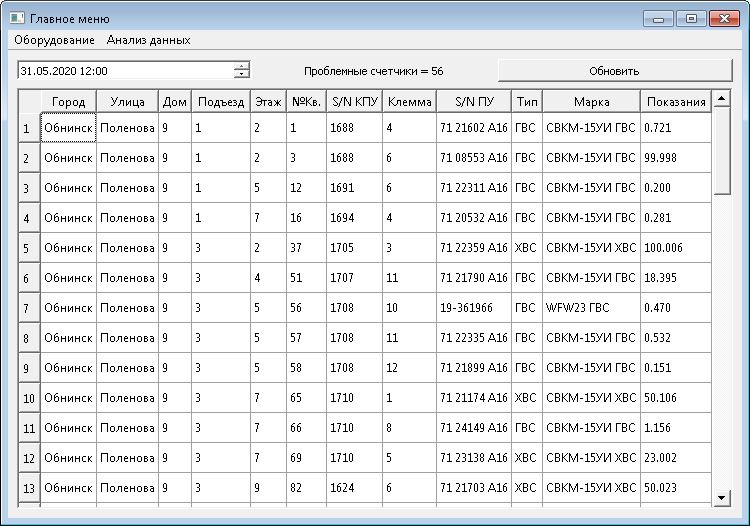
\includegraphics[width=0.7\linewidth]{pics/3}
	\caption{Список проблемных счетчиков}
	\label{fig:3}
\end{figure}
Проанализируем показания некоторых проблемных счетчиков.
По построенному графику видно, что счетчик горячей воды перестал работать 30 мая. (рисунок~\ref{fig:11})
\begin{figure}[H]
	\centering
	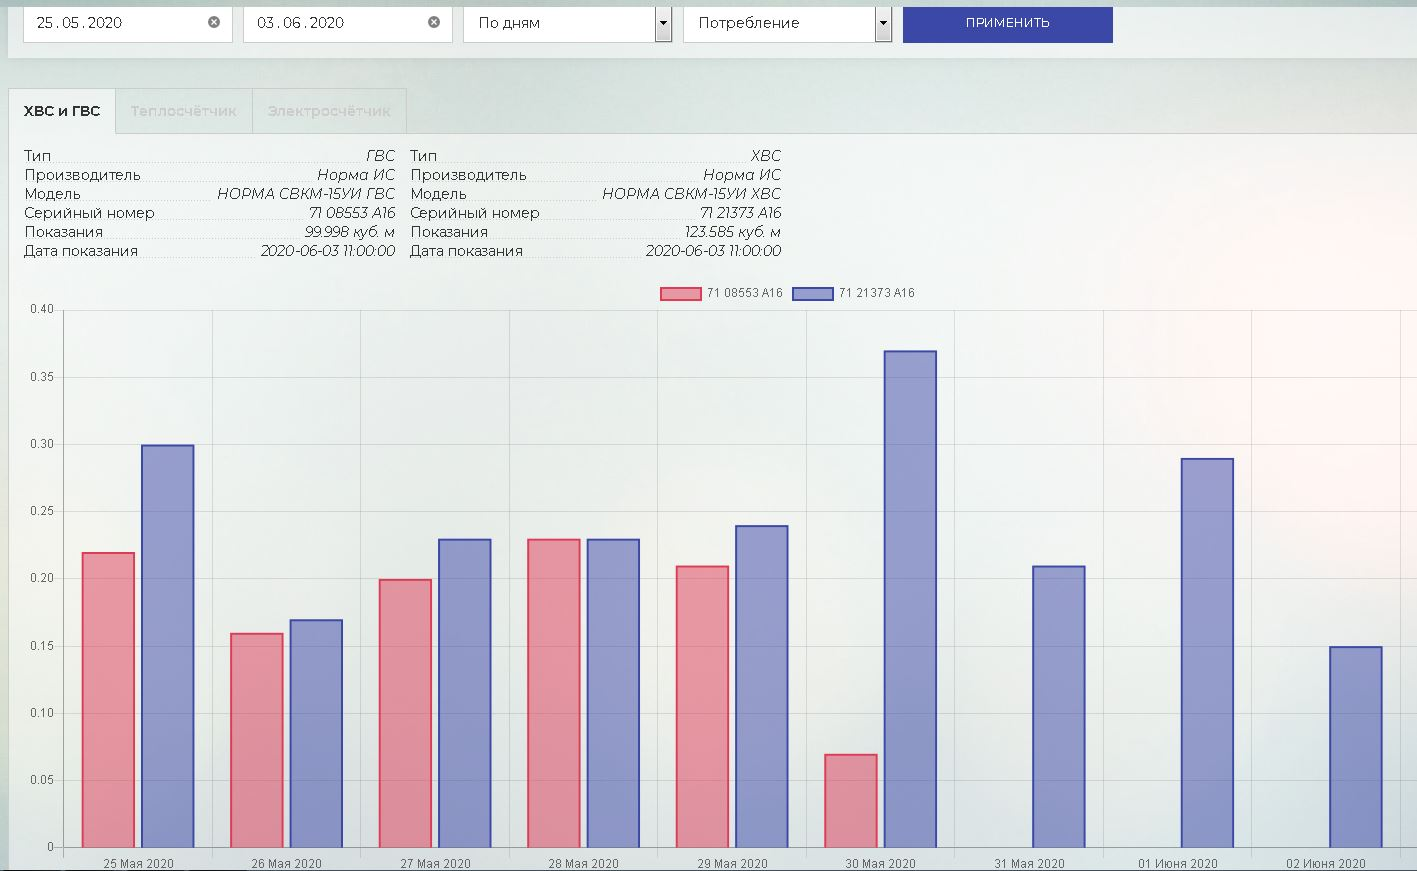
\includegraphics[width=0.7\linewidth]{pics/11}
	\caption{Поленова 11 кв.17}
	\label{fig:11}
\end{figure}
На графике (рисунок~\ref{fig:dom}) отображено потребление домового счетчика холодного водоснабжения в двух разных домах.
\begin{figure}[H]
	\centering
	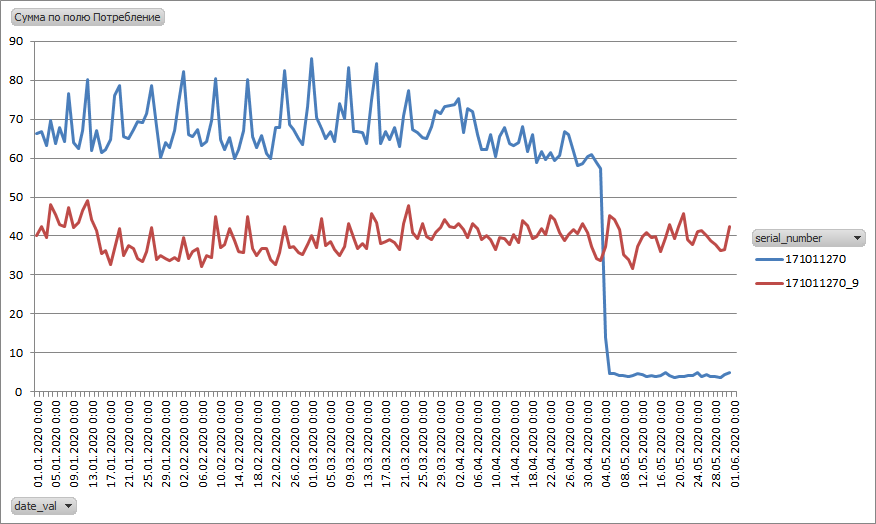
\includegraphics[width=0.7\linewidth]{pics/dom}
	\caption{Общедомовой счетчик воды}
	\label{fig:dom}
\end{figure}
По неизвестным причинам 4 мая сильно уменьшилось потребление холодной воды у одного из домов. Счетчик начал неверно отображать показания. Для точности посмотрим показания этого счетчика взятые из базы данных, таблица~\ref{tab:tab4}.
\begin{table}[H]
\caption{Потребление домового счетчика воды} \label{tab:tab4}
\centering
\begin{tabular}{|c|c|c|}
	\hline 
	Дата & Показания & Потребление \\ 
	\hline 
	02.05.2020 & 30059,53 & 58,86 \\ 
	\hline 
	03.05.2020 & 30118,39 & 57,23 \\ 
	\hline 
	04.05.2020 & 30175,62 & 14,05 \\ 
	\hline 
	05.05.2020 & 30189,67 & 4,83 \\ 
	\hline 
	06.05.2020 & 30194,5 & 4,58 \\ 
	\hline 
	07.05.2020 & 30199,08 & 4,18 \\ 
	\hline 
\end{tabular} 
\\Источник: собственные данные
\end{table}

В ходе проверки проблемных счетчиков, выяснилось, что отбор таких счетчиков проходит грубо. 17 счетчиков оказались рабочими, просто их потребление не подходит под стандартный анализ данных.

Скриншоты работы программы представлены в приложении Б, частичный код программы представлен в приложении В.